\begin{frame}
  \frametitle{Assumptions}

  \begin{itemize}
  
  \item New Nuclear = Advanced Boiling Water Reactors.
  
  \item Simplistic, conservative assumption about demand growth = +1.7\% per year.
  
  \item Nuclear, wind, solar annual growth rate \textbf{limits} based on trends in USA, China, Japan.
  
  \item CCS: Available for deployment in 2030, costs reduce by 2050.
  
  \item Offshore and onshore wind capacity limited to theoretical potential (about 450 GW and 200 GW respectively).
  
  \item H$_2$: Steam reforming available in 2030, photocatalytic conversion in 2050.
  
  \item Hydropower, geothermal capacity held constant.
  
  \end{itemize}

\end{frame}


\begin{frame}
  \frametitle{Levelized cost projections for solar and wind}
  \begin{figure}[htbp!]
    \begin{center}
      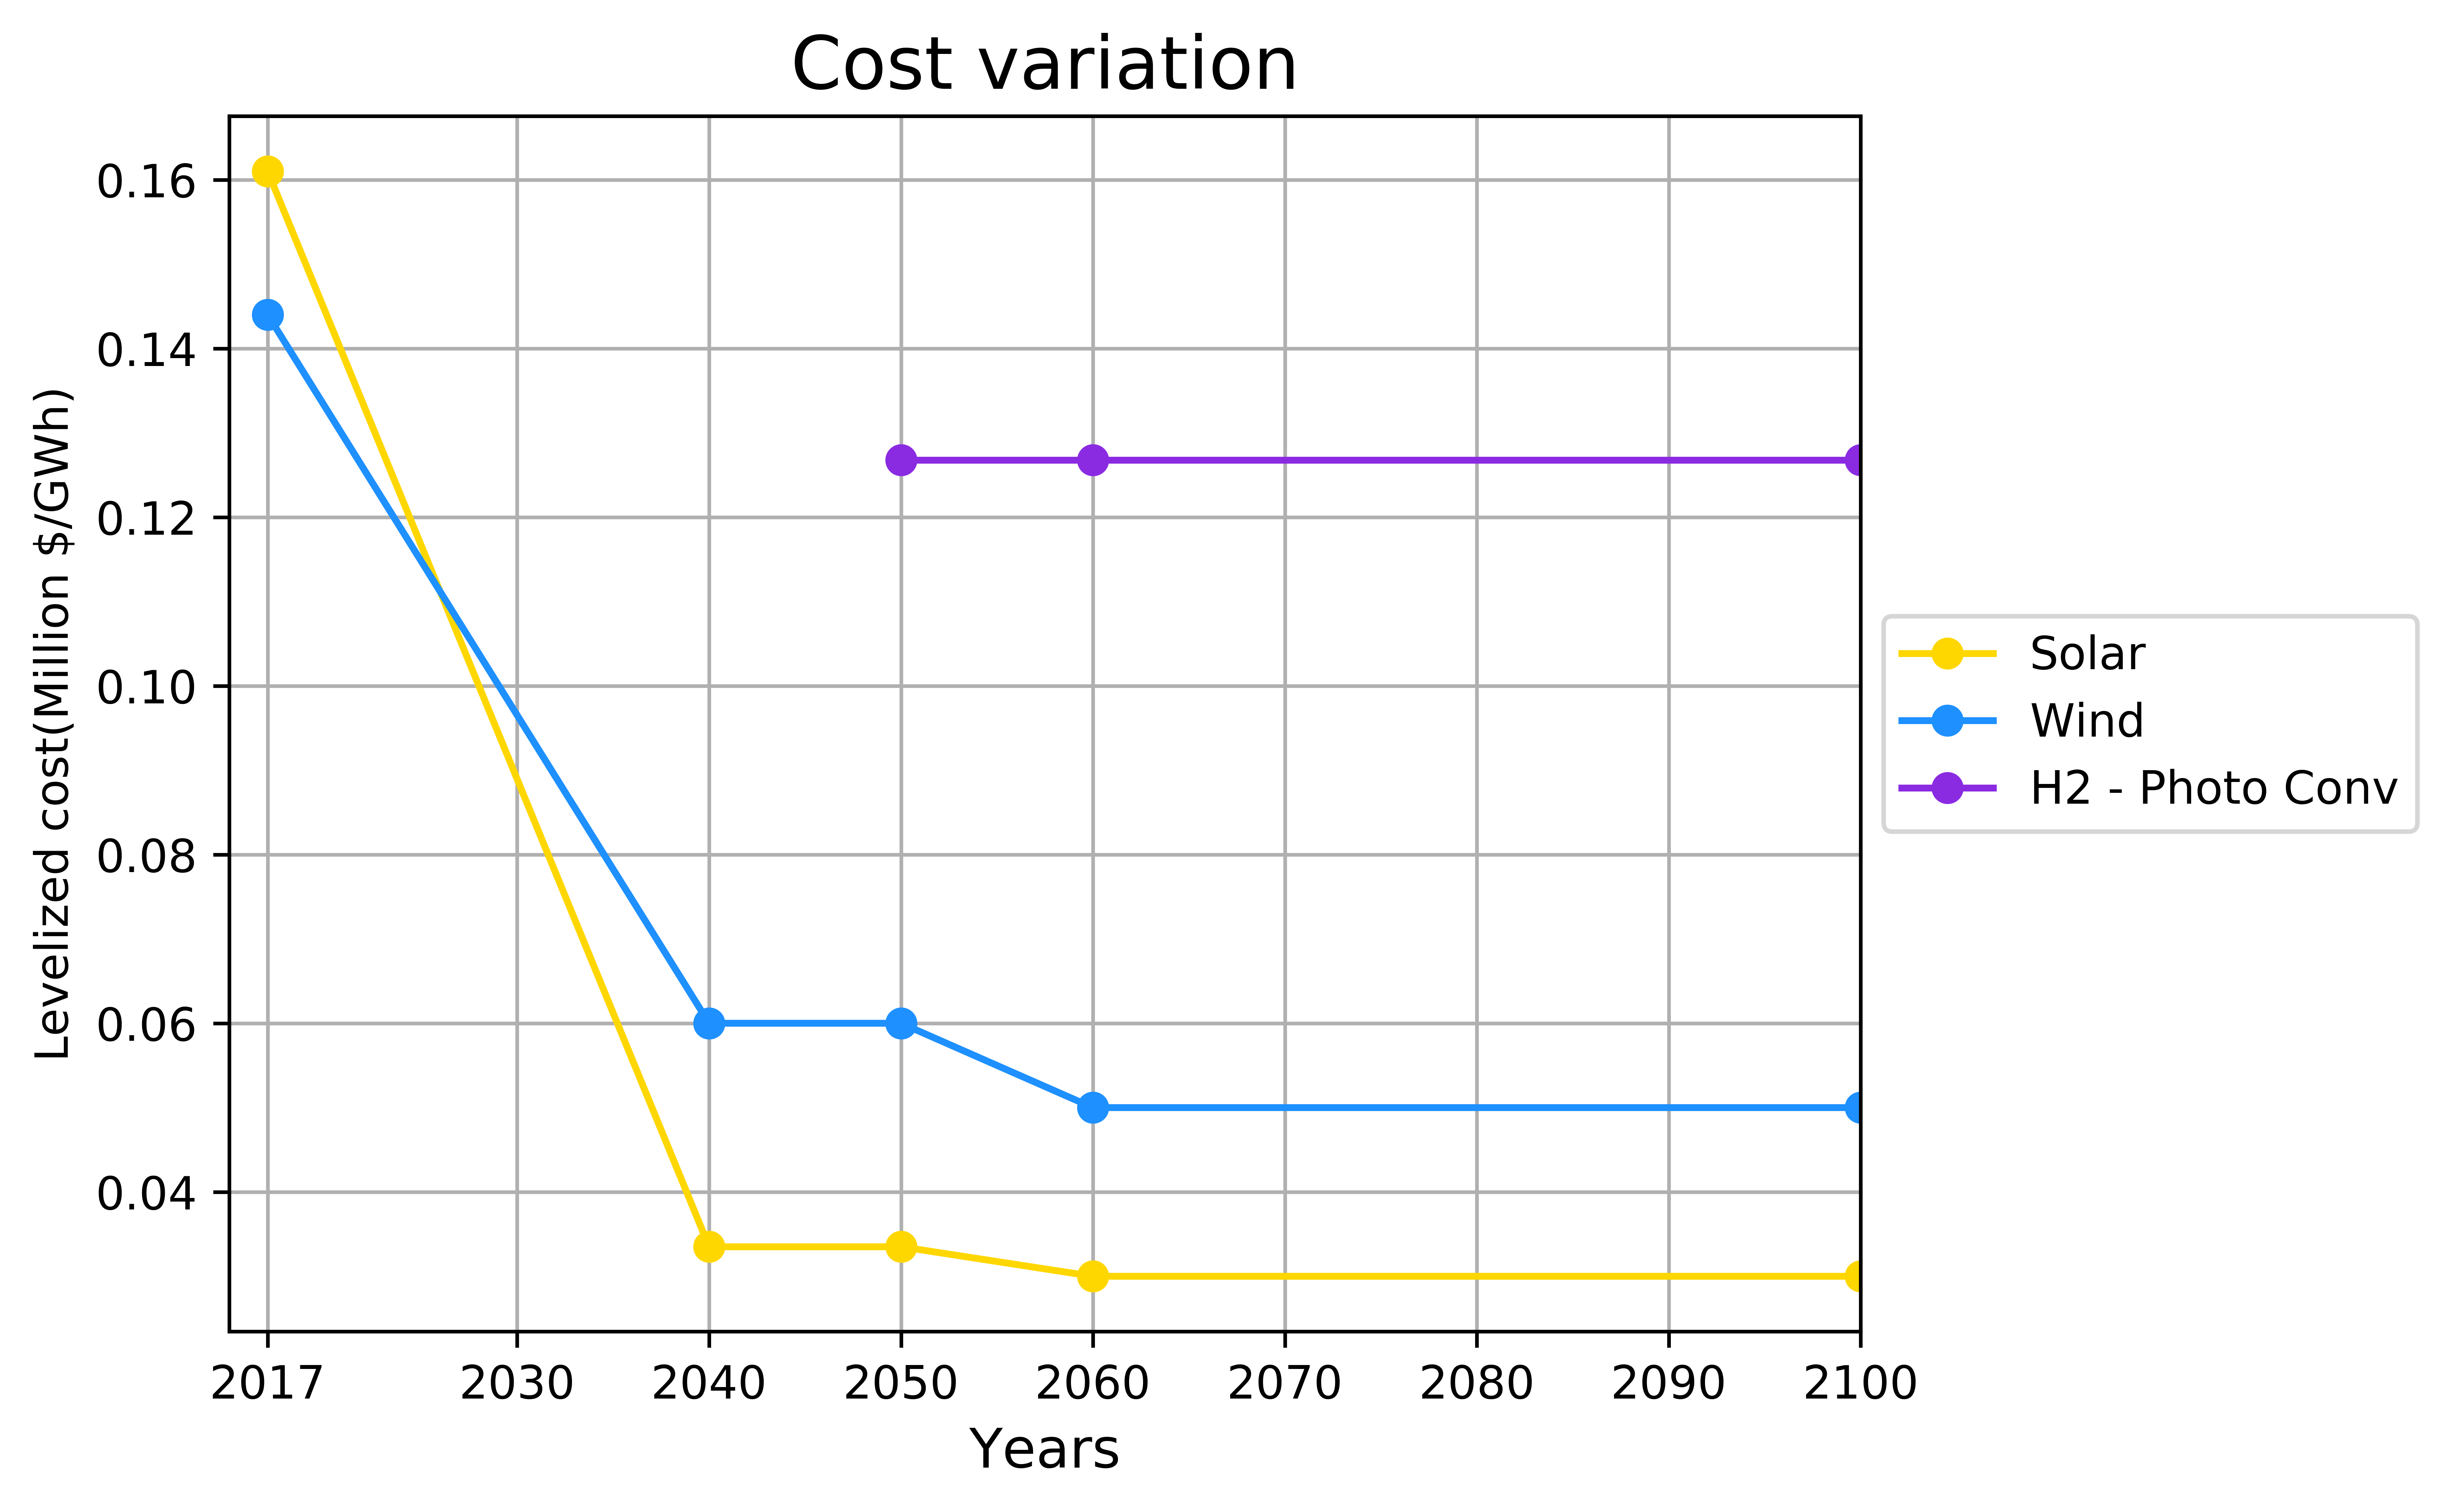
\includegraphics[scale=0.6]{./images/cost}
    \end{center}
          \caption{Cost variation of solar, wind, and H$_2$ production.}
    \label{cost}
  \end{figure}
\end{frame}

\begin{frame}
\frametitle{Contribution to peak factor (C2P factor}
This is a TIMES parameter that defines what fraction of a energy source's capacity is guaranteed to be available during peak demand.
\begin{tabular}{|c|c|}
\textbf{Energy source} &
\textbf{C2P factor} \\
\hline 
Fossil fuels & 1 \\
Nuclear power & 1 \\
Solar power & 0.42 \\
Wind & 0.20 \\
\end{tabular}

This factor is reduced for solar and wind with increasing penetration.
\end{frame}